\begin{frame}
\frametitle{Numerical description}
\begin{itemize}
\item Verbal description is essential for understanding.
\item<2-> However this does not include quantitative or visual information.
\item<3-> A \emph{numerical} description gives output data for a relevant set of input data.
\item<4-> This facilitates construction/study of a mathematical model.
\item<5-> Numerical description is typically given by table.
\item<6-> This table contains numerical data collected through experiments at selected input levels. 
\end{itemize}
\end{frame}

\begin{frame}
\frametitle{Examples: describing multivariable function via numerical data.}
\begin{itemize}
\item the following is Wind Chill Chart provided by NOOA:
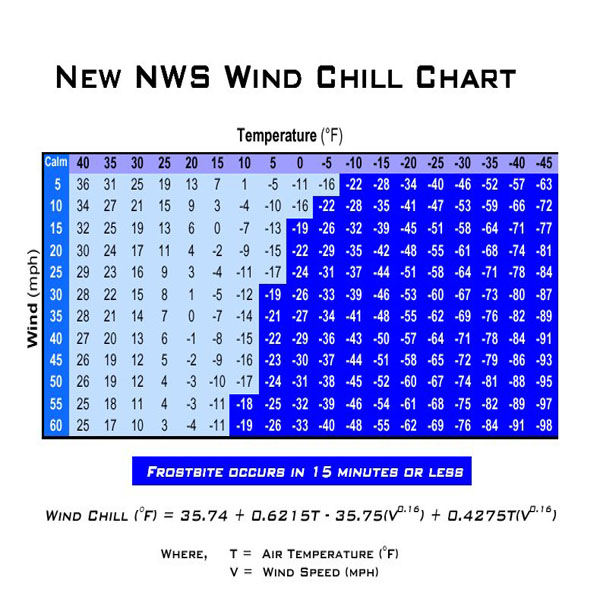
\includegraphics[width=3in]{../../modules/multivariable-functions/pictures/windchill2.jpg}
\end{itemize}
\end{frame}
\begin{frame}
\begin{itemize}
\item Another example is the Income Tax Table. Explain what the
input and output variables are in that case.
\end{itemize}
\end{frame}